% 基礎数学 第03回 ワークシート（CC BY-SA 4.0）
% 解答版は worksheet_answers.tex をビルドする
\documentclass[a4paper,11pt]{ltjsarticle}
\usepackage{lfs-worksheet}

\begin{document}
\lfsheader{基礎数学}{第03回 指数関数 ワークシート}

\problem{次の式を計算しなさい。(1)(2) は $a^{\square}$ の形に、(3)(4) は分数または整数で答えなさい（$a > 0$）。}
\begin{minipage}[t]{0.48\linewidth}
  (1) $a^3 \times a^5$
  \answerbox[2.4cm]{$a^{3+5} = a^8$}
  (3) $2^{-3}$
  \answerbox[2.4cm]{$\dfrac{1}{2^3} = \dfrac{1}{8}$}
\end{minipage}\hfill
\begin{minipage}[t]{0.48\linewidth}
  (2) $(a^2)^4 \div a^3$
  \answerbox[2.4cm]{$a^{8} \div a^3 = a^{8-3} = a^5$}
  (4) $3^0 + 4^{-1}$
  \answerbox[2.4cm]{$1 + \dfrac{1}{4} = \dfrac{5}{4}$}
\end{minipage}

\problem{次の値を求めなさい。(4) は指数の形に直してから計算しなさい。}
\begin{minipage}[t]{0.48\linewidth}
  (1) $8^{\frac13}$
  \answerbox[2.4cm]{$\sqrt[3]{8} = 2$ \quad （$2^3 = 8$ より）}
  (3) $16^{-\frac34}$
  \answerbox[2.4cm]{$16 = 2^4$ より $\left(2^4\right)^{-\frac34} = 2^{-3} = \dfrac{1}{8}$}
\end{minipage}\hfill
\begin{minipage}[t]{0.48\linewidth}
  (2) $27^{\frac23}$
  \answerbox[2.4cm]{$\left(\sqrt[3]{27}\right)^2 = 3^2 = 9$}
  (4) $\sqrt[3]{4} \times \sqrt[3]{2}$
  \answerbox[2.4cm]{$2^{\frac23} \times 2^{\frac13} = 2^{\frac23 + \frac13} = 2^1 = 2$}
\end{minipage}

\problem{右の図は、指数関数 $y = a^x$（$a > 0$、$a \neq 1$）のグラフで、点 $(2,\,9)$ を通る。}
\begin{minipage}[t]{0.56\linewidth}
  (1) 底 $a$ の値を求めなさい。
  \answerbox[2.4cm]{$a^2 = 9$、$a > 0$ より $a = 3$}
  (2) $x = -1$ のときの $y$ の値を求めなさい。
  \answerbox[2.4cm]{$y = 3^{-1} = \dfrac{1}{3}$}
\end{minipage}\hfill
\begin{minipage}[t]{0.4\linewidth}
  \vspace{2mm}
  \begin{center}
    % ワークシート問3：y = a^x のグラフ（2点 (0,1)・(2,9) を通る。a = 3）（CC BY-SA 4.0）
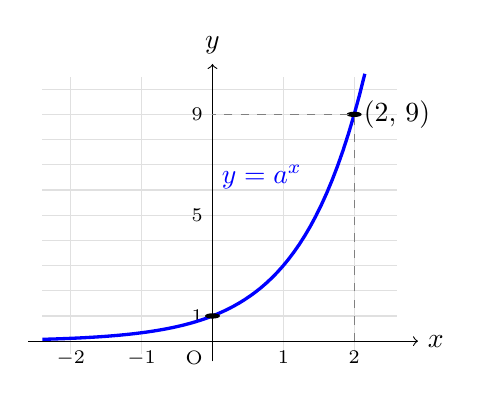
\begin{tikzpicture}[xscale=0.9,yscale=0.32]
  \draw[step=1,black!12,yscale=1] (-2.4,-0.5) grid (2.6,10.5);
  \draw[->] (-2.6,0) -- (2.9,0) node[right] {$x$};
  \draw[->] (0,-0.8) -- (0,11) node[above] {$y$};
  \foreach \t in {-2,-1,1,2} \node[below,font=\scriptsize] at (\t,0) {$\t$};
  \node[below left,font=\scriptsize] at (0,0) {O};
  \foreach \t in {1,5,9} \node[left,font=\scriptsize] at (0,\t) {$\t$};
  \draw[very thick,blue,domain=-2.4:2.15,samples=60] plot (\x,{3^\x});
  \fill (0,1) circle (3pt);
  \fill (2,9) circle (3pt) node[right] {$(2,\,9)$};
  \draw[dashed,black!50] (2,0) -- (2,9) -- (0,9);
  \node[blue,left] at (1.4,6.5) {$y = a^x$};
\end{tikzpicture}

  \end{center}
\end{minipage}

\problem{3つの数 $\sqrt{2}$，\ $\sqrt[3]{4}$，\ $\sqrt[5]{8}$ を、底を $2$ にそろえて、小さい順に並べなさい。}
\answerbox[4.5cm]{%
  $\sqrt{2} = 2^{\frac12}$，\quad $\sqrt[3]{4} = 2^{\frac23}$，\quad $\sqrt[5]{8} = 2^{\frac35}$\\[1ex]
  指数を通分すると $\dfrac12 = \dfrac{15}{30}$，\ $\dfrac23 = \dfrac{20}{30}$，\ $\dfrac35 = \dfrac{18}{30}$ \quad より \quad $\dfrac12 < \dfrac35 < \dfrac23$\\[1ex]
  底 $2 > 1$ なので \quad $\sqrt{2} < \sqrt[5]{8} < \sqrt[3]{4}$}

\problem{ある薬の成分は、体内での量が3時間ごとに半分になる（半減期3時間）。はじめに $80$ mg あったとき、$t$ 時間後の量は $m(t) = 80 \left(\dfrac12\right)^{\frac{t}{3}}$ mg と表せる。}
\begin{minipage}[t]{0.48\linewidth}
  (1) 6時間後の量を求めなさい。
  \answerbox[3cm]{$m(6) = 80 \left(\dfrac12\right)^{2} = 80 \times \dfrac14 = 20$\\[1ex]
  答え：$20$ mg}
\end{minipage}\hfill
\begin{minipage}[t]{0.48\linewidth}
  (2) 量が $10$ mg になるのは何時間後か。
  \answerbox[3cm]{$\left(\dfrac12\right)^{\frac{t}{3}} = \dfrac{10}{80} = \dfrac18 = \left(\dfrac12\right)^3$\\[1ex]
  より $\dfrac{t}{3} = 3$ \quad 答え：$9$ 時間後}
\end{minipage}

\end{document}
